\chapter{Design}\label{ch:design}
% The main part of your thesis. Here you describe your approach to solve
% the problem you stated in the Introduction.  Be as general as possible.

\section{Context} % Where does the design live?
As stated in \cref{ch:introduction}, packet-level \gls{fec} protects a flow against loss by
transmitting redundant, encoded packets alongside the original data. To do so, the encoder
must operate on a full \emph{generation} of packets belonging to the same flow before it can
produce repair packets. In a system that serves many concurrent flows at line rate, packets
of different flows arrive interleaved on a single ingress port, while the encoder consumes
them per-flow and in fixed-size groups. \\

This mismatch between the arrival order (interleaved,
per-packet) and the consumption order (per-flow, per-generation) is the central problem this
design addresses: a packet buffer that decouples packet arrival from encoder consumption by
storing packets in a shared memory pool and tracking their location with lightweight,
per-flow queues of descriptors, following the shared-memory architecture introduced in
\ref{ch:background}. This buffer sits between the ingress packet parser and the \gls{fec}
encoder in the overall pipeline, and is the sole subject of this thesis; the encoder itself
and anything downstream of it are outside its scope.

\subsection{System requirements}\label{system_requirements}
Based on the context above, the design should satisfy the following requirements:
\begin{itemize}
  \item Throughput of 100 Gb/s to achieve the line rate set by the Ethernet MAC
  \item Packet latency of under 10 $\mu$s (without accounting for buffering time) to let the \gls{fec} encoder dominate
  \item Configurable number of flows at compile time
  \item Configurable generation size at compile time
  \item Configurable queue length (both free memory and flow queues) at compile time
\end{itemize}

\subsection{Throughput and latency}
Of the requirements above, throughput and latency are the two that drive the architecture the
most directly: the buffer must sustain 100 Gbit/s line rate set by the Ethernet
\gls{cmac}, and it must add no more than 10 $\mu$s of latency so
that the \gls{fec} encoder's own processing time dominates the end-to-end delay budget. It is important 
to remark that actual packet latency (time difference from packet ingress to egress) is mostly determined 
by the input pattern as it seen in \ref{ch:evaluation}. This is caused by the fact that given a generation 
size of A, we need to wait for A packets from a given flow to arrive before feeding them to the encoder, 
which does not depend on the packet buffer itself. Instead, the requirement above refers to the time 
required for a packet to go through the whole datapath without accounting for the idle time it is 
waiting in the queues. \\

The remaining requirements (configurable flow count, generation 
size, and queue depths) are primarily parameterization choices rather than architectural 
drivers, and are discussed as such in \cref{subsec:assumptions}. How the design in this 
chapter is dimensioned and pipelined to meet the throughput and latency targets is detailed 
further in \cref{ch:implementation}.

\subsection{Assumptions and constraints}\label{subsec:assumptions}
The design presented in this chapter is validated exclusively through behavioural simulation; no
hardware synthesis, place-and-route, or on-board testing is performed as part of this
thesis. Consequently, features that are only needed for deployment such as configuration registers, which 
would expose the configurable parameters at runtime, are considered out of scope and are
not implemented. \\

Instead, every configurable parameter (flow count, generation size, and
queue depths) is fixed at elaboration time. The result should therefore be understood as a
baseline platform that provides a starting point onto which features can later be added 
without changing the core architecture. That being said, the proposed design can 
be synthesized as-is and should allow to statically test a future complete SmartNIC system. \\

The design is meant to be fully configurable, but some core decissions require a plausible 
target workload.  Based on measurements reported in \cite{alizadeh2010dctcp},
on the order of 30 to 40 flows can be expected to require concurrent \gls{fec} protection at any given time in a
representative deployment. Using this as a start reference point, the following example configuration is used
to evaluate the design. It has intentionally been chosen to be on the larger side, in order to
stress the design: \\

\begin{table}[h]
  \centering
  \begin{tabular}{ll}
    \hline
    Parameter & Value \\
    \hline
    Generation size            & 32 \\
    Number of flows            & 128 \\
    Free memory queue depth    & 1024 \\
    Flow (packet) queue depth  & 64 \\
    \hline
  \end{tabular}
  \caption{Example configuration used throughout this thesis}\label{tab:example-config}
\end{table}

The flow (packet) queue depth of 64 is set to twice the generation size, so that a full
generation can be accumulated for one flow while the previous generation is still being
drained by the read engine, without stalling ingest. The 128 supported flows aims to give 
the configuration leaves considerable headroom against the assumed 30 to 40 concurrent flows 
as stated in \cite{alizadeh2010dctcp}. \\

This configuration also embeds a simplifying assumption: the flow ingest stage
(\cref{sec:flow-ingest}) currently maps every tracked flow to exactly one dedicated flow
queue. Supporting more concurrent flows than there are queues (e.g. by having
several flows share a single queue) is not possible in the current design, but would only require
extending the tuple table inside flow ingest to map multiple flow IDs onto the same queue
index; the rest of the datapath is agnostic to this mapping and would not need to change.

\section{System design}
As covered in the background chapter \ref{ch:background}, the design is built with a shared-memory architecture. 
Figure \ref{fig:overall_system} depicts a high-level architectural view of the system. The subsequent 
sections break down the different stages roughly following the order of the datapath. \\

\begin{figure}
  \begin{center}
    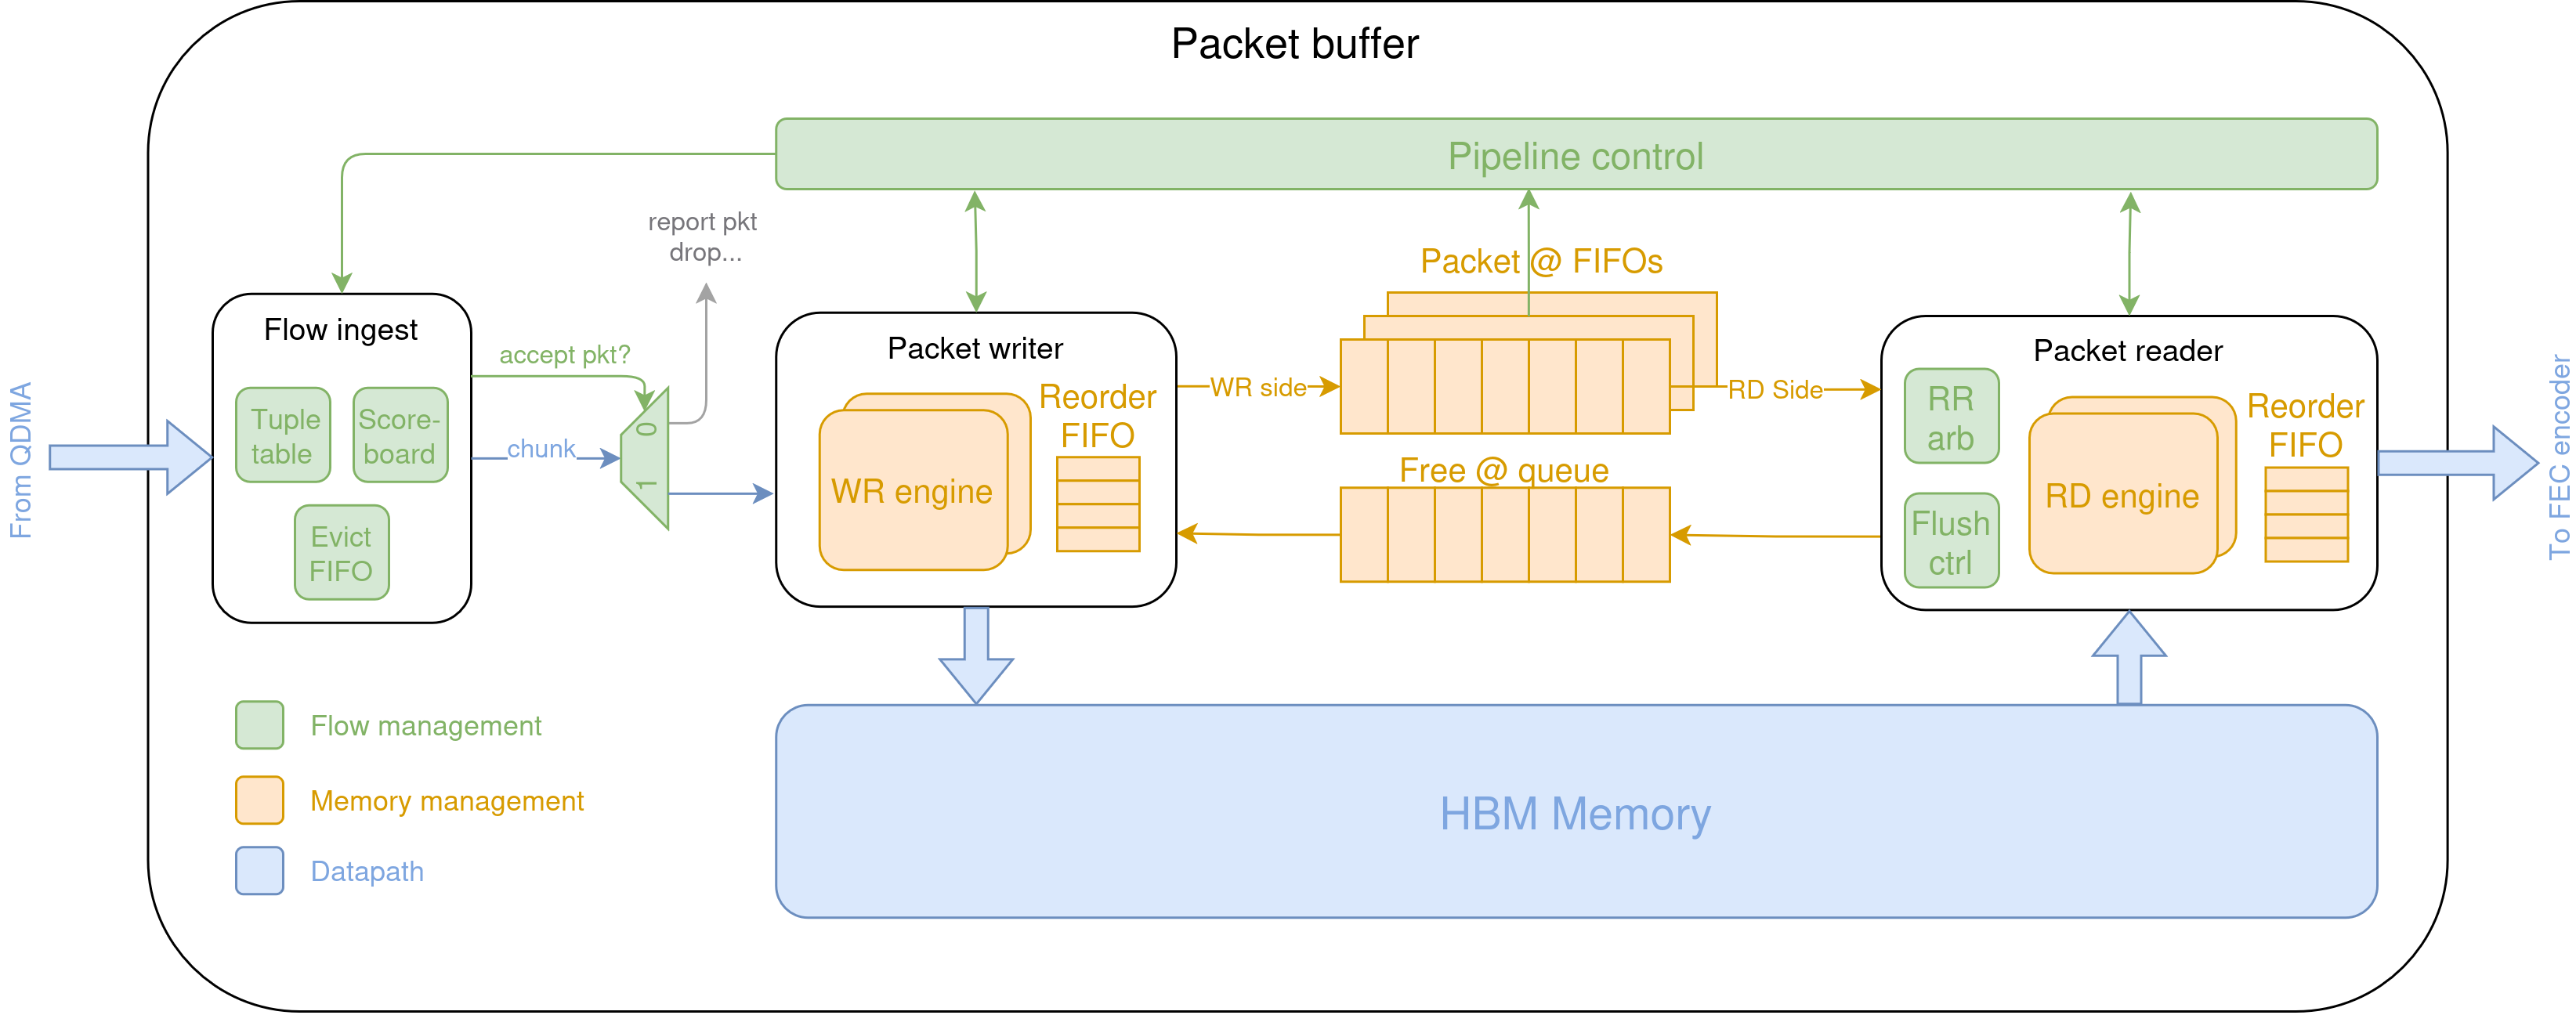
\includegraphics[width=1\textwidth]{../img/overall_system.png}
  \end{center}
  \caption{Overview of the Packet Buffer}\label{fig:overall_system}
\end{figure}

The packet payloads themselves are held in a single pool of \gls{hbm}, shared across all
flows; none of the control-path stages described below ever move or copy packet data
directly. Instead, every stage after ingest operates on lightweight descriptors (an
\gls{hbm} address together with the packet length and its internal flow ID) so that the
scheduling, queueing, and buffer-management logic can run at a much smaller data width and
higher effective rate than the 100 Gbit/s packet stream itself.

\subsection{Flow ingest}\label{sec:flow-ingest}
This is the first stage in the datapath, and its purpose is to allocate the internal resources
to the incoming flows, and tracking the state of said flows. This functions are split into three 
different modules:

\begin{itemize}
    \item \textbf{Flow ID table}: Maps the tuple identifying an incoming flow to a compact
    internal flow ID. Every packet that enters the system carries this tuple; rather than
    propagating it through the rest of the datapath, the flow ID table performs a lookup on
    ingest and replaces it with a small, fixed-width flow ID that is carried alongside the 
    descriptor from this point onward. This keeps every downstream structure (scoreboard, 
    packet queues, packet writer and packet writer) indexed and sized by flow ID 
    rather than by the much wider original tuple.
    \item \textbf{Flow metadata table}: Holds the per-flow state needed to service a flow once
    it has been assigned an ID, indexed by that same flow ID. This includes per-flow state machine 
    deatiled further in the implementation chapter \ref{ch:implementation}, 
    and a counter that keeps track of packets inside the packet writer/reader.
    \item \textbf{Evict ID queue}: A FIFO of flow IDs that are currently free and available
    for re-assignment. When a new tuple is seen for the first time, an ID is popped from this
    queue and assigned to it via the flow ID table. when a flow is torn down (evicted) because
    it has gone idle its ID is pushed back onto this queue, making it available for a future flow.
\end{itemize}

\subsection{Packet writer}
This stage takes in each incoming packet, together with the flow ID previously assigned to it, 
and is responsible for making that packet's payload visible to the rest of the
system as a descriptor. It first pops a free address from the free memory queue
(\cref{sec:descriptor-and-free-queues}) and uses it as the destination for the packet in the
shared \gls{hbm} pool, driving the necessary burst writes over \gls{axi}. \\

Once the write completes, the packet writer assembles a descriptor (the \gls{hbm} address 
just used, the packet length, and the flow ID) and pushes it onto the packet descriptor queue 
belonging to that flow. From this point on, the packet writer has no further involvement with the packet:
it is fully described by its descriptor until it is later read back out by the packet reader.

\subsection{Packet Descriptor and Free Memory queues}\label{sec:descriptor-and-free-queues}
These two sets of queues implement the address-based bookkeeping that lets the shared
memory pool be treated as a set of independent per-flow queues, without ever physically
partitioning the memory itself. \\

\textbf{Packet descriptor queues} are a set of FIFO, one per supported flow, each
holding the descriptors of the packets belonging to that flow that have been written to
\gls{hbm} but not yet consumed by the encoder. The packet writer pushes onto the queue
selected by the packet's flow ID; the packet reader pops from a queue once it has been
selected for service, in groups of the configured generation size. \\

\textbf{The free memory queue} is a single FIFO, shared across all flows, holding the
addresses of \gls{hbm} buffer slots that are not currently in use. It is initialized at reset
with every available address in the shared pool. The packet writer pops one address from it
per incoming packet, and the packet reader pushes an address back onto it once that packet
has been forwarded to the \gls{fec} encoder and its buffer slot can be reused. Because this
queue is shared rather than per-flow, buffer capacity is allocated on demand to whichever
flows are currently active, instead of being statically divided among all supported flows 
the central efficiency argument for a shared-memory architecture, as discussed in
\cref{ch:background}.

\subsection{Packet reader}
This stage is responsible for feeding the \gls{fec} encoder with complete generations of
packets, one flow at a time. An arbiter within the packet reader selects, from among the
flows whose packet descriptor queue currently holds at least a full generation of entries,
which flow to service next. Once a flow has been selected, the packet reader pops exactly
one generation's worth of descriptors from that flow's queue, and for each descriptor issues
the corresponding \gls{axi} read burst(s) against the address it contains, streaming the
retrieved payload out towards the \gls{fec} encoder together with its length and flow-ID
metadata. As each packet finishes being read out, its \gls{hbm} address is returned to the
free memory queue, making that buffer slot available for a new incoming packet.

\subsubsection{Internal vs external memory (\gls{hbm} usage justification)}
One of the first questions regarding system dimensions is the amount of required memory. Based on the aforementioned 
requirements in \ref{system_requirements}, we would like to support a generation size of 64
and at least 128 concurrent active flows. Assuming a worst case size of 1500 bytes per packet, and a packet queue of minimum size
(64 since we have to buffer at least as many packets as needed by the generation size); the resulting minimum memory is 12.288 MB
assuming perfectly efficient memory usage as seen in the calculation below.

\[
\begin{aligned}
\text{Memory}
&= 64\,\frac{\text{packets}}{\text{flow}}
\times 128\,\text{flows}
\times 1500\,\frac{\text{bytes}}{\text{packet}} \\[4pt]
&= 12{,}288{,}000\,\text{bytes} \\[4pt]
&= \frac{12{,}288{,}000}{10^6}\,\text{MB} \\[4pt]
&= \boxed{12.288\,\text{MB}}
\end{aligned}
\]
According to the product page of the Alveo U55C board \cite{amd_alveo_u55c}, the total SRAM capacity is roughly 42 MB, of which only
around 33 come from the denser UltraRam memory in Xilinx FPGAs. Since the goal of this design is to be potentially scalable to handle
hundreds of concurrent flows in the future, building around such a limited pool of storage is not acceptable. \\

Moreover, the memory is distributed across the FPGA fabric, and assembling it all together would likely require an internal network
that would also use a high amount of resources; introducing high wire delays due to the additional routing and greatly increasing 
overall system complexity.\\

Because of this, the logical decision is to make use of the external memory of the FPGA, which in the U55C's case is the 16 GB worth
of \gls{hbm}.


\subsubsection{Coherency and consistency}

In computer science and multi-core hardware, coherence ensures that all processors see the latest
written value for a single specific memory address, and consistency defines the global order
in which read and writes across different memory addresses appear to execute for all processors.\\

The proposed design does not contain any traditional processor cores, however it does contain two
modules (the packet reader and packet writer) that issue and handle multiple in-flight requests each,
raising the question about how to guarantee the coherency and consistency.\\

Thankfully, one of the biggest advantages of a shared-memory architecture is that the free memory and packet
queues guarantee that a packet descriptor can only be at one place at any given time: it is either
being processed in the write or read engine, or stored in one of the queues. This ensures that there can only
be exactly one request in flight (either a read or a write) for every memory address at any time.\\

In summary, as long as the write and read engines only pop and push to the queues only when memory
transactions have been completed, coherency and consistency are guaranteed.\\


% \subsection{System architecture}
% Add diagram of whole system, say that it looks like a shared memory system etc...
%
% Give a short walk through the datapath and say it will be elaborated later on.
%
% \subsection{Memory architecture}
% Super duper diagram indicating that we use a 
%
% \subsection{Flow ingest}
% Diagram + explanation of this stage.
%
% \subsection{Chunk ingest (packet writer)}
% Diagram + explanation of this stage.
%
% \subsection{Packet reader}
% Diagram + explanation of this stage.
%
% \subsection{Packet and memory queues}
% Diagram + explanation of this stage.

% \section{Previous \gls{hbm} architecture}\label{sec:prev_hbm_arch}
% Here I can speak (if William finds it appropriate) about the previous architecture without axi stream, since I already have the diagrams.

